% PhysicsLibrary submission source
% Suggested title: Free-body diagram
% Suggested entry type: Definition
% Suggested primary PACS classification: 45.20.Dd (Newtonian mechanics)
% Suggested additional classification: 45.50.Dd (General motion)
% Suggested synonyms: free body diagram, force diagram, FBD
% Suggested defines: system boundary, external force, internal force
% Suggested keywords: Newton's laws, force, free-body diagram, normal force,
% friction, tension, spring force, drag force, equilibrium, circular motion
% License intent: CC BY-SA 4.0

\section*{Free-body diagram}

A \emph{free-body diagram} (FBD) is a diagram in which one chosen object or system is isolated
from its surroundings and every relevant \emph{external} force acting on that object or system is
represented explicitly.  The purpose of an FBD is analytical rather than artistic: it separates
the object of interest from distracting geometric detail and provides the force model from which
Newton's equations are written.

For a particle or translating rigid body of constant mass,
\[
\sum \mathbf F_{\mathrm{ext}}=m\mathbf a.
\]
For a rigid body the same diagram also supplies the forces and moment arms used in rotational
dynamics,
\[
\sum \boldsymbol\tau_O=\frac{d\mathbf L_O}{dt},
\]
or, in an appropriate fixed-axis special case,
\[
\sum\tau=I\alpha.
\]

The most important word in the definition is \emph{chosen}.  Before drawing force arrows, one must
decide what object or collection of objects is the system.  Whether a force is external or internal
depends on this system boundary.

\section{System boundary}

A \emph{system boundary} separates the chosen system from everything else.  Forces exerted across
the boundary by the surroundings are external and belong on the free-body diagram.  Forces between
parts of a multi-body system are internal and normally do not appear on a free-body diagram of the
whole system.

For example, consider two blocks tied together.  If only one block is selected, the string tension
must appear on that block's FBD.  If both blocks are selected together, the tension is internal to
the two-block system and disappears from the system-level FBD.  Choosing a useful system boundary
is therefore an important problem-solving strategy.

\section{A seven-step construction procedure}

A reliable free-body diagram can be constructed by the following sequence.
\begin{enumerate}
\item \emph{Choose the system.} State whether the system is one particle, one rigid body, or several bodies treated together.
\item \emph{Sketch the isolated body.} For particle translation, a point or simple box is usually sufficient.
\item \emph{Identify every interaction crossing the system boundary.}
\item \emph{Replace each interaction by a force vector acting on the chosen system.}
\item \emph{Label forces by physical origin}, for example $m\mathbf g$, $\mathbf N$, $\mathbf T$, or $\mathbf f$.
\item \emph{Choose coordinate axes} that simplify the component equations.
\item \emph{Write Newton's equations only after the diagram is complete.}
\end{enumerate}

A useful final question is: ``For every force arrow, what body in the surroundings exerts this
force on the chosen system?''  If that question cannot be answered, the arrow may not represent a
real interaction.

\section{Forces commonly appearing on free-body diagrams}

\subsection*{Weight}

Near the surface of Earth,
\[
\mathbf W=m\mathbf g,
\]
directed approximately toward the center of Earth.  Weight should not be replaced by components
until coordinates have been selected.  On an incline, $mg\sin\theta$ and $mg\cos\theta$ are
components of one gravitational force, not additional forces.

\subsection*{Normal force}

A normal force is a contact force perpendicular to a surface.  Its magnitude is not automatically
$mg$.  It must be determined from the equations of motion and the geometry of contact.

\subsection*{Tension}

An ideal flexible string or cable pulls along its own direction.  In the common ideal model of a
massless string over frictionless massless pulleys, the tension magnitude is the same throughout a
continuous string.

\subsection*{Friction}

Friction acts tangentially to a contact surface and opposes relative sliding or the tendency to
slide.  Static friction satisfies
\[
|f_s|\leq \mu_sN,
\]
whereas a common kinetic-friction model is
\[
f_k=\mu_kN.
\]
The equality $f_s=\mu_sN$ applies only at impending slip.

\subsection*{Spring force}

For an ideal linear spring,
\[
\mathbf F_s=-k\mathbf x,
\]
where the minus sign indicates a restoring force.

\subsection*{Drag}

Common approximations are
\[
\mathbf F_d=-b\mathbf v
\]
for linear drag and
\[
\mathbf F_d=-c|\mathbf v|\mathbf v
\]
for quadratic drag.

\section{Forces are not their components}

Suppose an applied force of magnitude $F$ makes angle $\theta$ with the positive $x$-axis.  One may
write
\[
\mathbf F=F\cos\theta\,\hat{\mathbf i}+F\sin\theta\,\hat{\mathbf j}.
\]
The component terms are a representation of the same force; they are not additional interactions.
The same warning applies to the components of weight on an inclined plane.

\section{Newton's third law and FBDs}

Newton's third law states
\[
\mathbf F_{A\to B}=-\mathbf F_{B\to A}.
\]
The two forces act on different bodies and therefore do not normally appear together on a single
body's free-body diagram.  For a book on a table, the table's normal force on the book and the
book's weight are not a third-law pair because both forces act on the book.

\section{Coordinate choices}

Good axes simplify the equations.
\begin{itemize}
\item For horizontal surfaces, horizontal and vertical axes are usually natural.
\item For inclined planes, axes parallel and perpendicular to the plane are usually best.
\item For circular motion, radial and tangential directions are often most useful.
\end{itemize}

No separate ``centripetal force'' should be added in an inertial frame.  Centripetal force means the
radial component of the net real force,
\[
\sum F_r=m\frac{v^2}{r}.
\]

\section{Diagram gallery}

The following diagrams use external figure files together with ordinary \verb|\includegraphics|.
The files are stored in the accompanying \verb|figures/| directory so that PhysicsLibrary's
LaTeX/latex2html workflow can render them without relying on TikZ or the LaTeX \verb|picture|
environment.

\subsection{Hanging mass}
\begin{figure}[h]
\centering
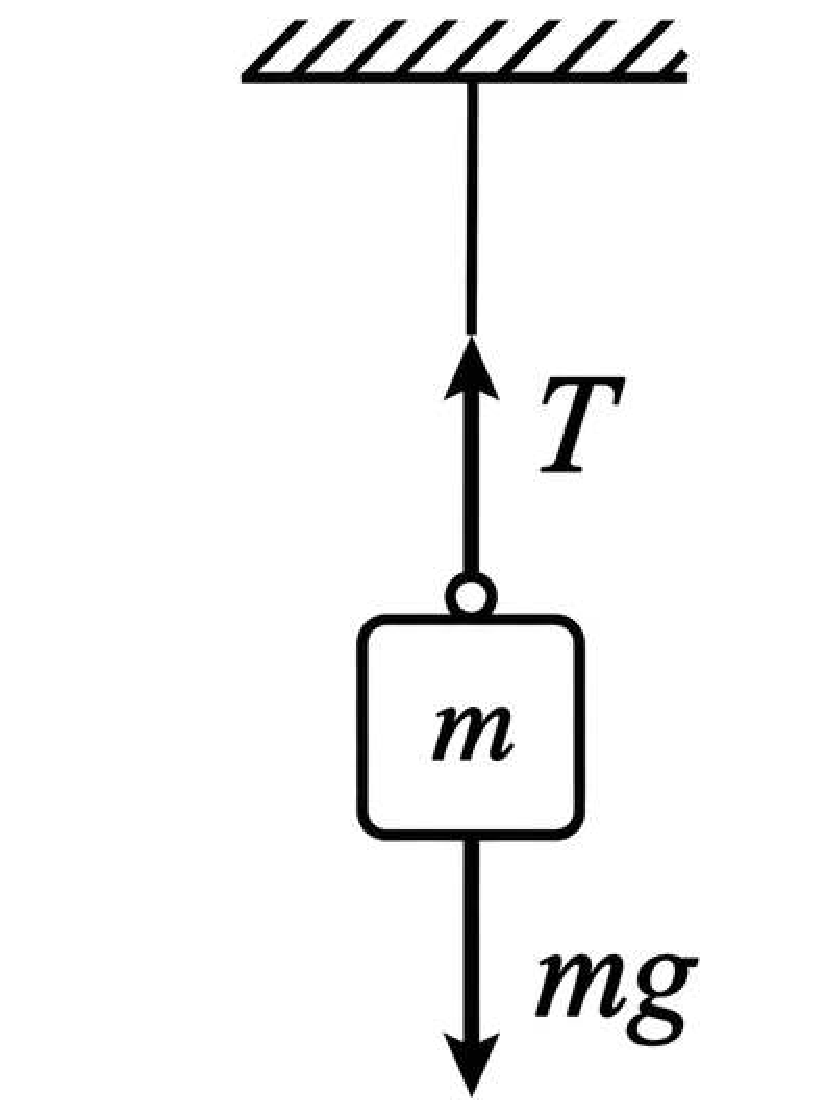
\includegraphics[width=0.34\textwidth]{figures/hanging_mass_free_body_diagram}
\caption{A hanging mass with upward tension and downward weight.}
\end{figure}

For a hanging mass attached to a light string,
\[
T-mg=ma_y.
\]

\subsection{Block on a horizontal surface}
\begin{figure}[h]
\centering
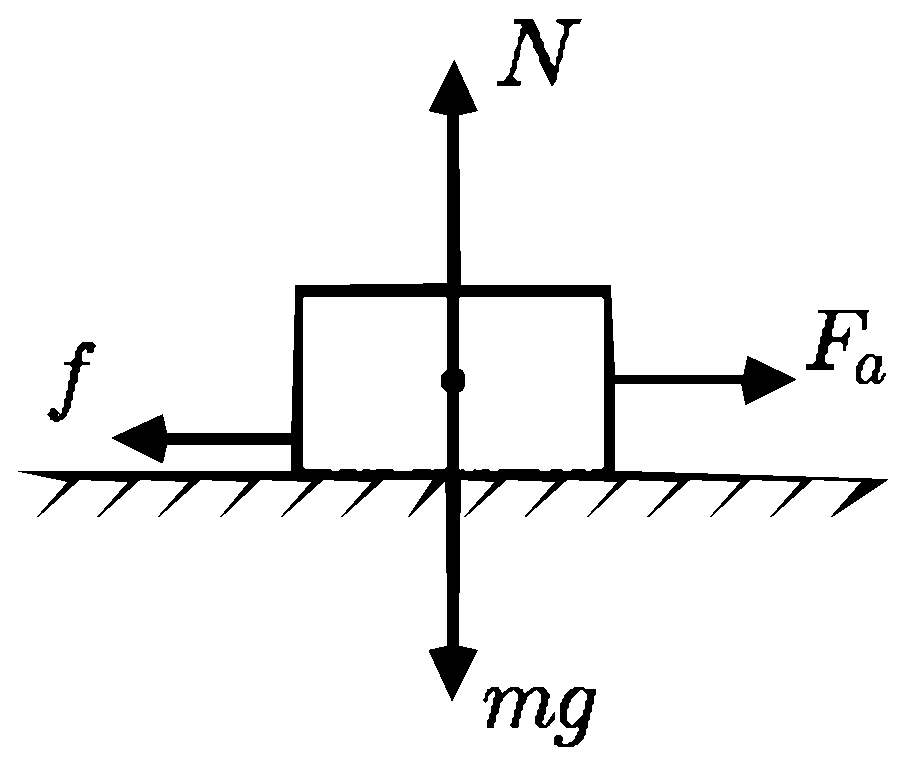
\includegraphics[width=0.55\textwidth]{figures/minimalist_free_body_diagram}
\caption{A rough horizontal surface with applied force, friction, normal force, and weight.}
\end{figure}

If vertical acceleration is zero,
\[
N-mg=0,
\]
and if the block slides,
\[
F_a-f_k=ma,
\qquad
f_k=\mu_kN.
\]

\subsection{Block on an inclined plane}
\begin{figure}[h]
\centering
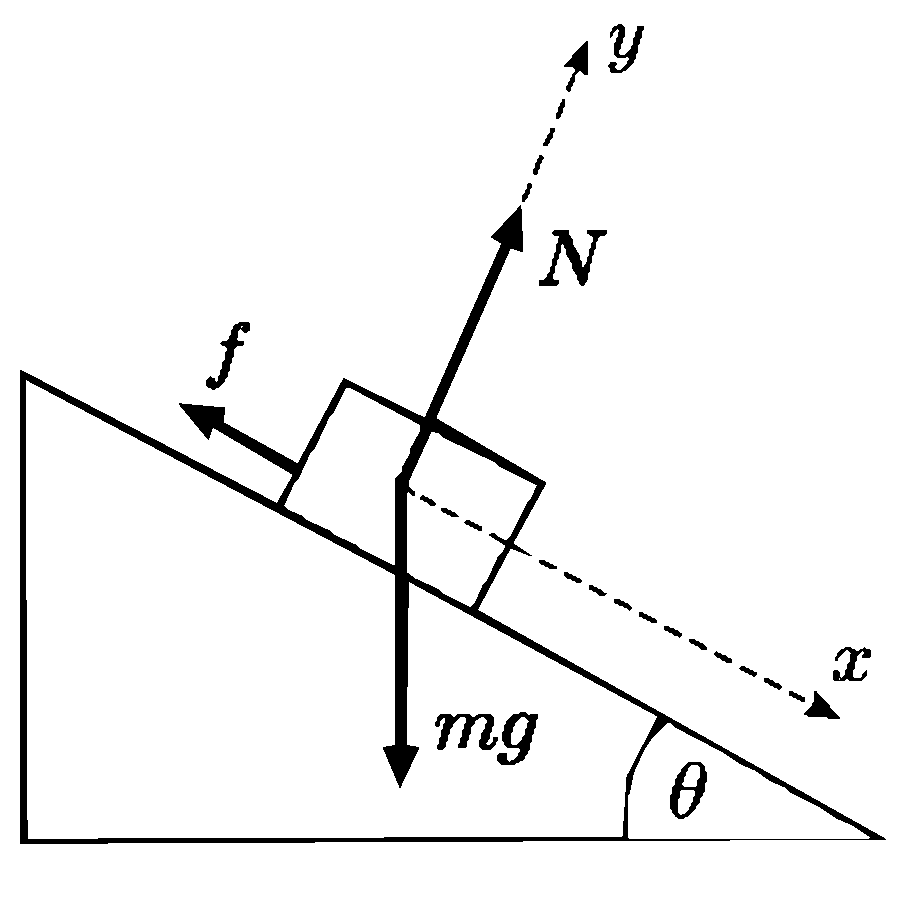
\includegraphics[width=0.56\textwidth]{figures/inclined_plane_free_body_diagram}
\caption{A block on an inclined plane.}
\end{figure}

With axes parallel and perpendicular to the plane,
\[
W_{\parallel}=mg\sin\theta,
\qquad
W_{\perp}=mg\cos\theta.
\]

\subsection{Rough-surface block pulled at an angle}
\begin{figure}[h]
\centering
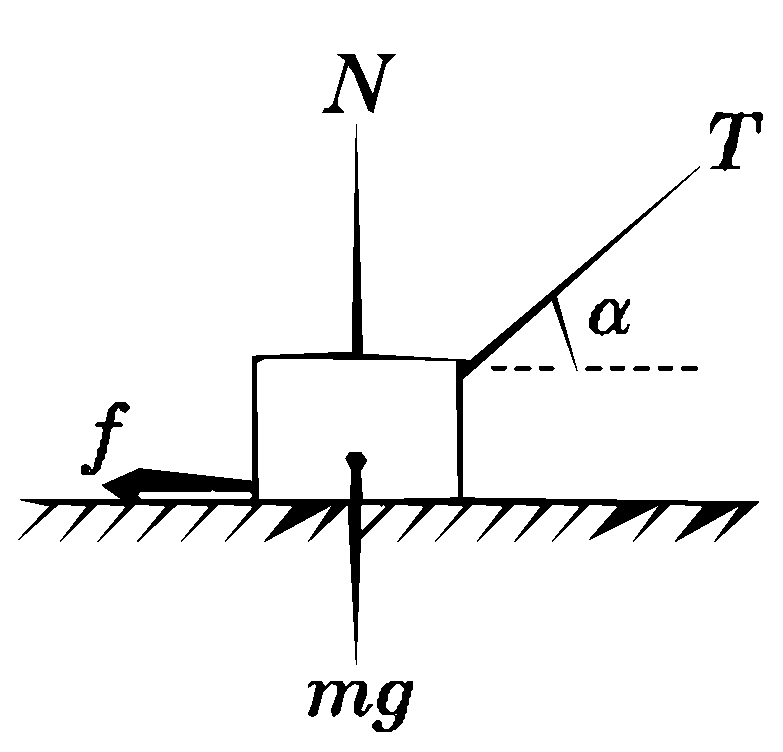
\includegraphics[width=0.56\textwidth]{figures/free_body_diagram_of_a_rough_surface_block}
\caption{A rough-surface block pulled by an oblique force.}
\end{figure}

The vertical component of the pull changes $N$ and therefore changes the friction magnitude.

\subsection{Block against a vertical wall}
\begin{figure}[h]
\centering
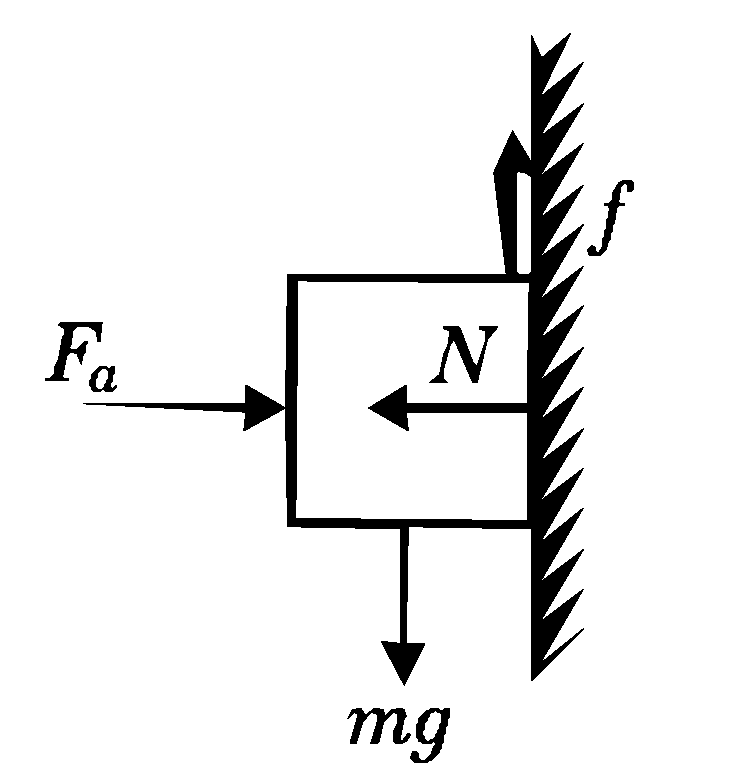
\includegraphics[width=0.48\textwidth]{figures/free_body_diagram_of_block_against_wall}
\caption{A block held against a vertical wall.}
\end{figure}

If the block tends to slide downward, static friction acts upward.

\subsection{Mass-spring system}
\begin{figure}[h]
\centering
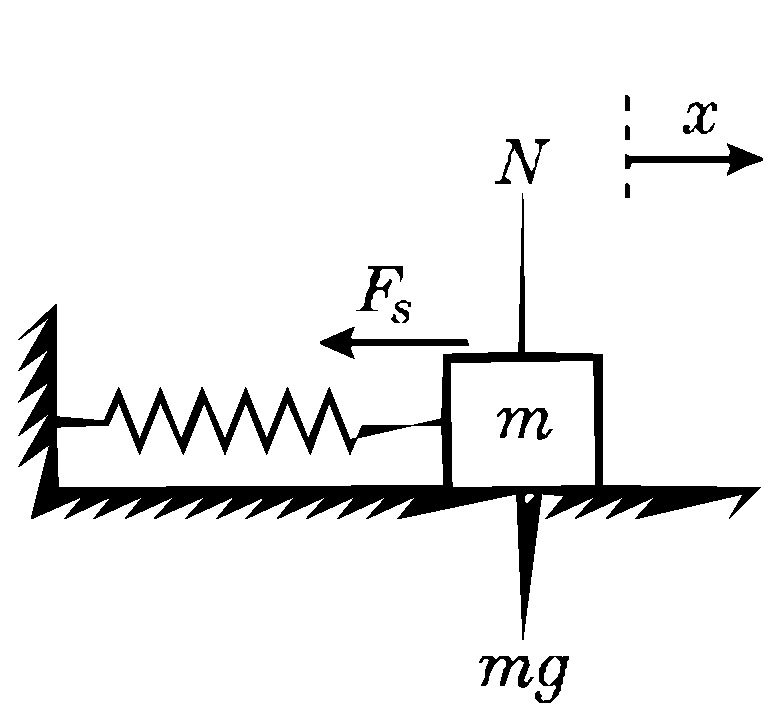
\includegraphics[width=0.58\textwidth]{figures/mass_spring_free_body_diagram}
\caption{A horizontal mass-spring system.}
\end{figure}

For an ideal spring,
\[
F_s=-kx.
\]

\subsection{Pendulum bob}
\begin{figure}[h]
\centering
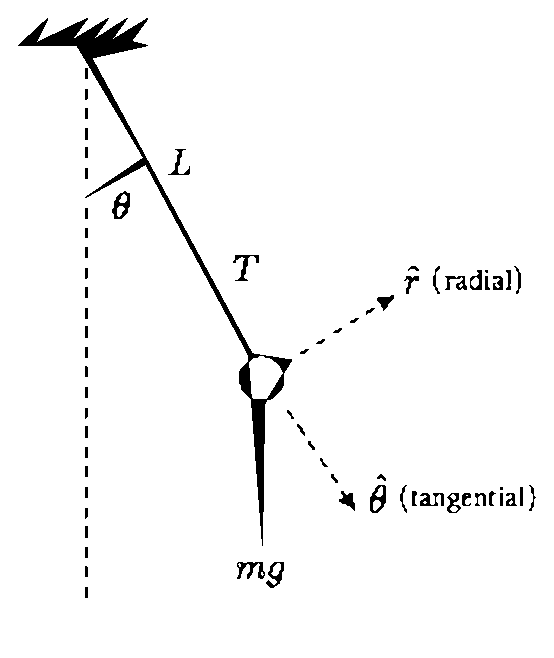
\includegraphics[width=0.50\textwidth]{figures/pendulum_free_body_diagram}
\caption{A pendulum bob with tension and weight.}
\end{figure}

Radial and tangential directions are especially convenient for pendulum dynamics.

\subsection{Banked curve}
\begin{figure}[h]
\centering
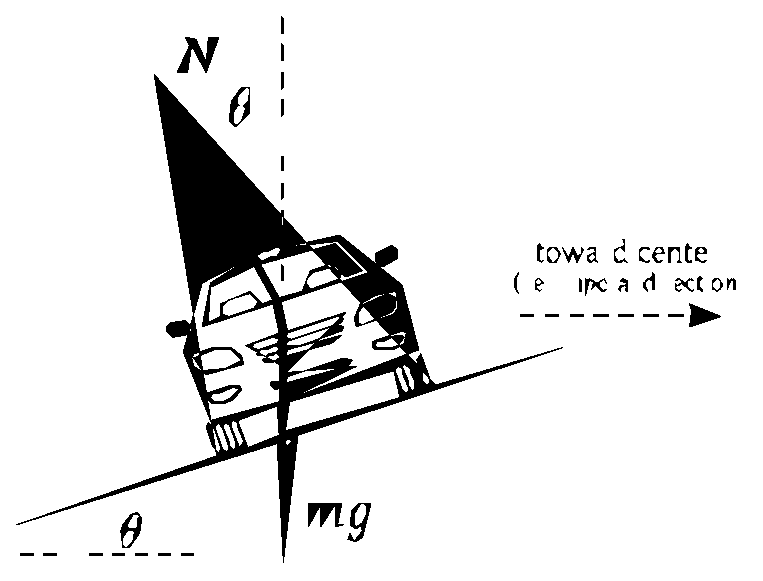
\includegraphics[width=0.60\textwidth]{figures/banked_curve_free_body_diagram}
\caption{A vehicle represented on a banked curve.}
\end{figure}

The normal force need not be vertical; its horizontal component can contribute to centripetal
acceleration.

\subsection{Loop-the-loop at the top}
\begin{figure}[h]
\centering
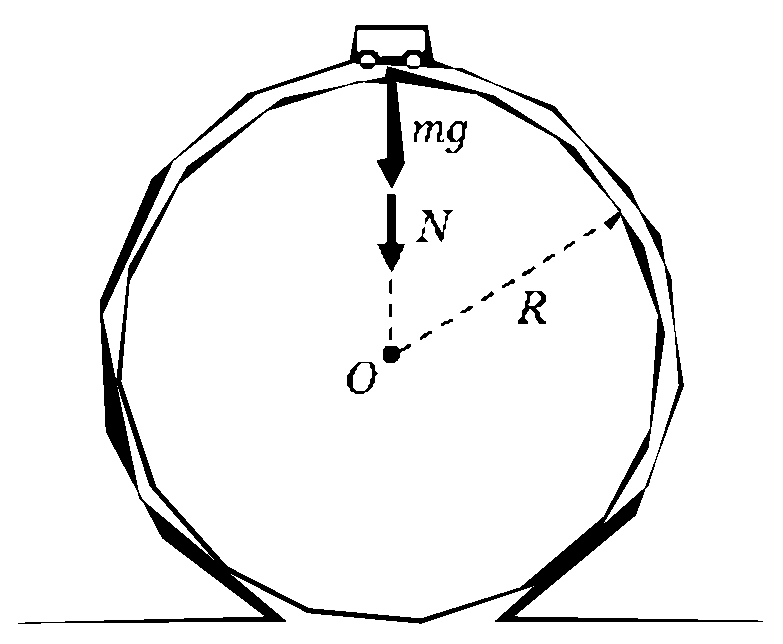
\includegraphics[width=0.56\textwidth]{figures/loop_the_loop_force_diagram}
\caption{At the top of an inside loop, both $N$ and $mg$ point toward the center.}
\end{figure}

The radial equation is
\[
N+mg=m\frac{v^2}{r}.
\]

\subsection{Atwood machine}
\begin{figure}[h]
\centering
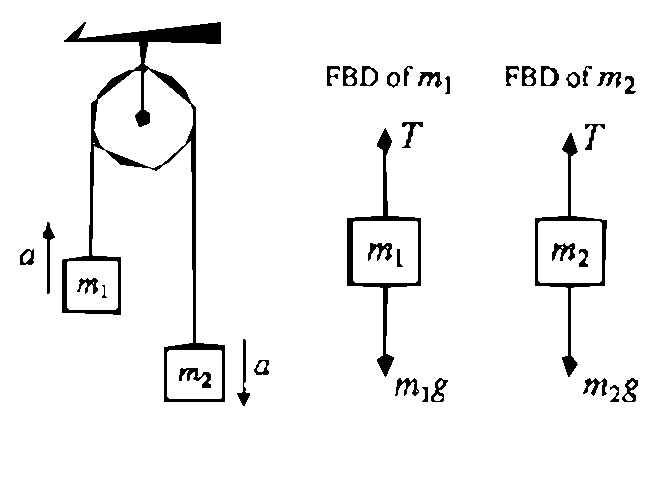
\includegraphics[width=0.82\textwidth]{figures/atwood_machine_free_body_diagrams}
\caption{An Atwood-machine system sketch and separate FBDs for the two masses.}
\end{figure}

For $m_2>m_1$ and an ideal string and pulley,
\[
T-m_1g=m_1a,
\]
\[
m_2g-T=m_2a,
\]
so
\[
a=\frac{(m_2-m_1)g}{m_1+m_2}.
\]

\section{Worked examples}

\subsection*{Example 1: horizontal pull}

A $5.0\,\mathrm{kg}$ block is pulled horizontally by a $20\,\mathrm{N}$ force on a frictionless
horizontal surface.  The FBD gives
\[
20=5.0a,
\qquad
N-5.0g=0.
\]
Hence
\[
a=4.0\,\mathrm{m/s^2},
\qquad
N=49\,\mathrm{N}.
\]

\subsection*{Example 2: pull at an angle}

A $10\,\mathrm{kg}$ block is pulled with force $50\,\mathrm{N}$ at $30^\circ$ above horizontal.
The vertical equation is
\[
N+50\sin30^\circ-mg=0,
\]
so
\[
N=mg-25\,\mathrm{N}.
\]
If kinetic friction is present, its magnitude is $\mu_kN$, showing why the vertical component of an
oblique pull changes the horizontal friction force.

\subsection*{Example 3: frictionless incline}

For a block on a frictionless incline of angle $\theta$,
\[
mg\sin\theta=ma,
\qquad
N=mg\cos\theta,
\]
so
\[
a=g\sin\theta.
\]

\subsection*{Example 4: rough incline}

If a block slides down a rough incline,
\[
mg\sin\theta-f_k=ma,
\qquad
f_k=\mu_kmg\cos\theta,
\]
therefore
\[
a=g(\sin\theta-\mu_k\cos\theta).
\]

\subsection*{Example 5: terminal speed with linear drag}

For downward positive direction,
\[
mg-bv=m\frac{dv}{dt}.
\]
At terminal speed, $dv/dt=0$, hence
\[
v_t=\frac{mg}{b}.
\]

\subsection*{Example 6: car at the top of a loop}

At the top of an inside loop, inward is downward.  The real inward forces are $N$ and $mg$:
\[
N+mg=m\frac{v^2}{r}.
\]
The minimum speed for contact occurs when $N=0$,
\[
v_{\min}=\sqrt{gr}.
\]

\section{Common mistakes}

\begin{enumerate}
\item Omitting an external interaction.
\item Adding a force that acts on another body rather than the chosen body.
\item Drawing both members of a Newton's-third-law pair on one body's FBD.
\item Drawing both a force and its components as separate forces.
\item Treating ``centripetal force'' as an extra force.
\item Assuming $N=mg$ without checking the vertical or normal equation.
\item Assuming static friction always equals $\mu_sN$.
\item Choosing axes that make the geometry unnecessarily complicated.
\end{enumerate}

\section{Practice exercises}

\begin{enumerate}
\item Draw the FBD for a lamp hanging from a single vertical cord.
\item Draw the FBD for a crate pushed across a rough horizontal floor.
\item Draw the FBD for a block sliding down a frictionless incline.
\item Draw the FBD for a block at rest on a rough incline.
\item Draw separate FBDs for the two masses in an Atwood machine.
\item Draw the FBD for a car rounding a flat circular turn.
\item Draw the FBD for a pendulum bob at angle $\theta$ from the vertical.
\item Draw the FBD for a block pressed against a vertical wall by a horizontal force.
\item Draw the FBD for a mass attached to a horizontal spring.
\item Draw the FBD for an object falling through a fluid with drag.
\item Draw the FBD for a car at the bottom of a vertical loop.
\item Draw the FBD for a car at the top of a vertical loop.
\item For two blocks tied together on a frictionless table, compare the FBD of one block with the FBD of the two-block system.
\item Explain why the normal force and weight of a book on a table are not a Newton's-third-law pair.
\end{enumerate}

\section{GRE-style speed checks}

The following original questions are intended to test rapid force-diagram reasoning.

\begin{enumerate}
\item A block rests on a horizontal table with no other vertical forces.  Which relation follows?\\
(A) $N>mg$ \quad (B) $N<mg$ \quad (C) $N=mg$ \quad (D) $N=0$\\
\emph{Answer: C.}

\item A car moves at constant speed around a flat circular curve.  Which real force can provide the inward acceleration?\\
(A) weight \quad (B) normal force \quad (C) static friction \quad (D) a separate centripetal force\\
\emph{Answer: C.}

\item A block is pulled upward at an angle on a horizontal floor.  Compared with an equal purely horizontal pull, the normal force is generally: \\
(A) larger \quad (B) smaller \quad (C) unchanged \quad (D) zero\\
\emph{Answer: B.}

\item At the top of an inside vertical loop, the inward direction is downward.  Which forces may point inward?\\
(A) $N$ only \quad (B) $mg$ only \quad (C) both $N$ and $mg$ \quad (D) neither\\
\emph{Answer: C.}

\item A block is static on a rough incline below the angle of impending slip.  Static friction is: \\
(A) always $\mu_sN$ \quad (B) whatever value is required up to $\mu_sN$ \quad (C) zero \quad (D) always downhill\\
\emph{Answer: B.}

\item Two masses form an ideal Atwood machine.  If both masses are chosen as one system, the string tension is: \\
(A) external \quad (B) internal \quad (C) gravitational \quad (D) a fictitious force\\
\emph{Answer: B.}

\item A book rests on a table.  Which is the third-law partner of the table's normal force on the book?\\
(A) the book's weight \quad (B) Earth's force on the table \quad (C) the book's force on the table \quad (D) friction\\
\emph{Answer: C.}

\item A block moves in a circle.  Which statement is correct?\\
(A) centripetal force must be drawn as an extra arrow \\
(B) centripetal force means the inward component of the net real force \\
(C) centripetal force is always gravity \\
(D) centripetal force is always tension\\
\emph{Answer: B.}
\end{enumerate}

\section{Non-inertial frames}

The diagrams above assume an inertial frame.  If Newton's second law is written directly in an
accelerating or rotating frame, inertial-force terms such as centrifugal and Coriolis forces may be
introduced.  They should be labeled explicitly as frame-dependent inertial terms rather than being
confused with physical interactions such as gravity or contact forces.

\section{Bridge to analytical mechanics}

Free-body diagrams are central to Newtonian mechanics because they make individual forces explicit.
In Lagrangian mechanics, ideal constraint forces can often be eliminated by choosing generalized
coordinates adapted to the constraints.  The conceptual progression is therefore
\[
\text{identify forces and constraints}
\longrightarrow
\text{choose coordinates adapted to the constraints}
\longrightarrow
\text{derive equations from }L=T-U.
\]
Free-body-diagram reasoning remains valuable even when the final equations are obtained from a
variational principle because it clarifies the physical interactions and constraint assumptions.

\section{Source and licensing note}

The core workflow of isolating a body and replacing surrounding interactions by external forces is
consistent with the openly licensed treatment in \emph{Mechanics Map}; the present entry substantially
expands that workflow for calculus-based physics, GRE review, rigid-body applications, and the
transition to analytical mechanics.  The worked examples, practice problems, GRE-style questions,
and figure assets are original PhysicsLibrary material produced for this entry.

\begin{thebibliography}{9}

\bibitem{MechanicsMap}
J. Moore and contributors,
\emph{Mechanics Map}, Engineering LibreTexts.
Creative Commons Attribution--ShareAlike 4.0.
\PMlinkexternal{Mechanics Map}{https://eng.libretexts.org/Bookshelves/Mechanical_Engineering/Mechanics_Map_(Moore_et_al.)}

\bibitem{UCD}
T. Weideman,
\emph{UCD Physics 9A -- Classical Mechanics}, Physics LibreTexts.
Creative Commons Attribution--ShareAlike 4.0.
\PMlinkexternal{UCD Physics 9A}{https://phys.libretexts.org/Courses/University_of_California_Davis/UCD:_Classical_Mechanics}

\end{thebibliography}

Unless otherwise noted, this PhysicsLibrary entry is intended for release under the Creative Commons
Attribution--ShareAlike 4.0 International license.
